%license:BSD-3-Clause
%copyright-holders:Michele Maione
%============================================================
%
%	Cloud gaming platform for arcade games
%
%============================================================

\prefacesection{Abstract}
Il videogioco è un mezzo di intrattenimento unico che combina le diverse forme d'arte, quali musica, narrativa e animazione, all'interattività. Ed è proprio questa caratteristica che gli permette di esercitare un potenziale d'immersione e attrazione che gli altri media non hanno.

I videogiochi sono ormai diventati un fenomeno culturale di massa con centinaia di milioni di persone che giocano regolarmente ogni giorno, il che li rende un attore dominante nel settore dell'intrattenimento, settore in continua crescita che non ha mai subito interruzioni nel corso degli anni come mostrato in Fig. \ref{fig:valore_commerciale_giochi_globale}.

\begin{figure}[H]
	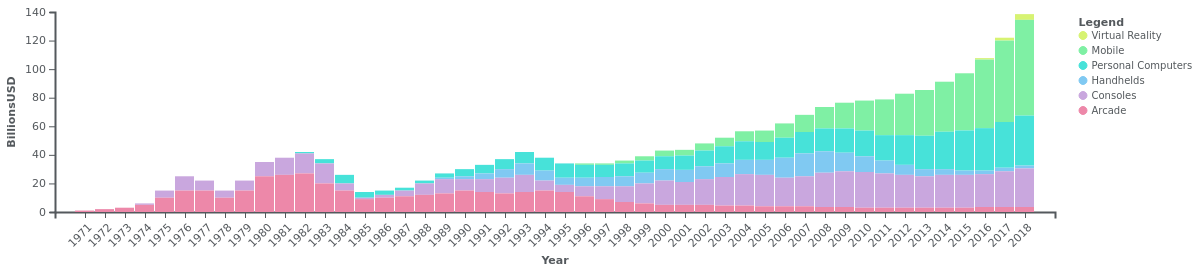
\includegraphics[width=\linewidth]{immagini/valore_commerciale_giochi_globale.png}
	\caption{Ricavi globali dell'industria dei videogiochi dal 1971 al 2018 (non adeguati all'inflazione). Fonte: wikipedia.org}
	\label{fig:valore_commerciale_giochi_globale}
\end{figure}

Con il continuo aumentare della velocità delle connessioni di rete, ci stiamo muovendo verso una nuova era digitale che influenzerà ogni aspetto della vita dei consumatori. La sfida consiste nell'inventare nuovi modelli di consumo dei contenuti e dei servizi esistenti, un'opportunità che si concretizza attraverso due tecnologie ormai entrate a far parte della vita di tutti i giorni: lo streaming e il cloud computing.

Questo progetto prevede la creazione di una piattaforma di cloud gaming, che permette lo streaming audio-video direttamente e su richiesta dei videogiochi, da un server remoto, ad un client (computer, console, telefono, tv). Il gioco è archiviato, eseguito, e renderizzato su un server remoto; l'input (tastiera, joystick) viene inviato dal client al server e lì processato.
In questo modo si può accedere ai giochi indipendentemente dal sistema operativo e dalle capacità hardware del client utilizzato. Inoltre il cloud gaming permette di iniziare a giocare immediatamente poiché il gioco è già installato sul server. Infine la piattaforma, indirettamente, garantisce la gestione dei diritti digitali (DRM) per gli editori.

Verrà ampliato il software MAME (rilasciato sotto licenza GNU-GPL), che è in grado di emulare  oltre 7.000 giochi arcade. Lo scopo di tale emulazione è quello di preservare la storia dei videogiochi e di prevenire la scomparsa di vecchie rarità una volta che le macchine originali abbiano cessato di funzionare per motivi di obsolescenza. La piattaforma sarà indipendente dal sistema operativo, rendendo più agevole l’installazione di uno stand per il retrogaming, ed insieme alla semplicità di accesso, attirerà le nuove generazioni e farà conoscere i giochi che hanno fatto la storia.

La tesi è strutturata come segue: nel Capitolo 1 viene introdotto il cloud gaming e fatta una panoramica dei servizi presenti sul mercato; si descrivono le tecnologie utilizzate nel Capitolo 2, mentre nel Capitolo 3 viene presentata l'architettura del sistema. All’interno del Capitolo 4 vengono illustrati i risultati ottenuti. Nell'ultimo capitolo sono riportate le conclusioni finali e una lista di possibili sviluppi futuri.